%%%%%%%%%%%%%%%%%%%%%%%%%%%%%%%%%%%%%%%%%%%%%%%%%%%%%%%%%%%%%%%%%%%%%%%%%%%%%%%%
%nscience.tex: Chapter on neutrino physics:
%%%%%%%%%%%%%%%%%%%%%%%%%%%%%%%%%%%%%%%%%%%%%%%%%%%%%%%%%%%%%%%%%%%%%%%%%%%%%%%%
%!TEX root = ../thesis_master.tex 
\chapter{Physics of \texorpdfstring{\Z}{Z} Transverse Momentum}
\label{chapter:theory}
\begin{figure}[!htbp]
    \centering
    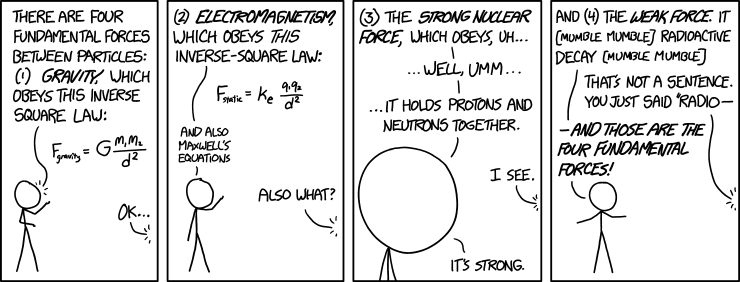
\includegraphics[width=\textwidth]{figures/TheoryFigures/fundamental_forcesXKCD.png}
    \caption[Short description of the four forces]{A \texttt{xkcd} comic explaining the four forces\cite{xkcdComic}}
    \label{fig:XKCDComic}
\end{figure}
\section{The Standard Model}
One of the most important aspects of science is to test the constituency of a theory, such as the case of the study of the mass of the W compared to the prediction of different models. Our current understanding of the fundamental constituents and forces of the physical world has developed through a continuous interplay between experimental observations and theoretical understanding.  The theoretical framework which encapsulates this process is called the Standard Model(SM), and benefits from major contributions from Weinberg, Glashow, Salam, and Higgs, as well as many others\cite{glashow1961,weinberg1967,salam1968,higgs1964}. The model is a relativistically-correct quantum field theory(QFT) that separates particles into two categories: fermions, which includes all matter (the most well known being the electron); and bosons, which are force carriers (an example of which is the photon, the force carrier of the electromagnetic force). The experiments have ranged in complexity from very simple experiments, such as the Rutherford's gold foil experiment\cite{rutherford1911} which showed that atoms have nuclei, to giant collider experiments, such as CMS, which discovered the Higgs boson. Despite the amount of effort that has gone into the production of the SM, it still is incomplete, with the most obvious missing piece being that it does not include the force of gravity. Within  a broad range of phenomena however, SM does an excellent job of describing particle physics as we are able to observe.


In particle physics, the definition of a force is different than the definition given to introductory physics students, $F=ma$. Instead, force is defined as something that allows the state of the particle to change. A change in momentum through attraction or repulsion is considered a force, but so too is a change in any other physical property, such as transforming into a different particle. When these forces are first explained to people the explanation tends to go like Fig \ref{fig:XKCDComic}. 


\section{The Electromagnetic Force}
Although, unlike the weak or strong nuclear force, the electromagnetic force does not directly have a major effect on the values of this thesis, but for completeness a section has been included. Unlike other forces, humans are able to directly detect the electromagnetic force using a specialized organ - our eyes - albeit in a very specific energy range. As a result, the nature of light has been a topic of debate for centuries. In the 17$^\text{th}$ century, Gassendi and Descartes put forward two competing and seemingly contradictory theories. Gassendi suggested that light was composed of beams of tiny particles, while Descartes argued that light was a wave, similar to those we see in water. Though both theories had supporters, Newton agreed with Gassendi that light was a particle. In part because of the weight of Newton's name, the majority of the scientific community followed the assumption that light was a particle for over a century. However, this opinion was challenged when later observations into diffraction were difficult to explain using the particle theory of light. One of these is the famous double slit experiment, wherein two slits are created on an opaque sheet and light is shone through it. When light passes through these slits, it creates a pattern of dark and light lines on a sheet behind it. This is in contrast to the expected result based on the particle theory, in which it would have created two bright spots. Later, Maxwell successfully described light as an electromagnetic wave, appearing to settle the debate in favor of the wave theory\cite{LightHistory}.\par
Near the beginning of the 20$^\text{th}$ century Max Planck studied black body radiation from a theoretical point of view. When using Maxwell's equations, an object should emit more energy at smaller wavelengths, with the amount of energy emitted asymptotically approaching infinity as the wavelength approaches zero.  This mathematical prediction has been dubbed the ``Ultraviolet Catastrophe." To match the theory with the experimental data, Plank found that radiation had to be emitted in quantized bunches with the form 
\begin{equation}\label{eq:PhotonEnergy}
    E
    =
    h\nu,
\end{equation}
where $E$ is the energy of the particle, $\nu$ is the frequency of the light and $h$ is a constant now commonly given his name\cite{ANDP:ANDP19013090310}. This put a minimum energy requirement on radiation in the high frequency range, rectifying the ultraviolet catastrophe. Einstein took this even further by stating that all light, not just light emitted from a black body, is quantized. This quantization became known as the photon. \par
	The contradiction between light being both a particle and a wave was resolved by the development of Quantum Field Theory (QFT), and specifically Quantum Electrodynamics (QED). QED describes electromagnetic interactions through the exchange of photons. Some simple examples are shown in Fig. \ref{fig:PhotonExamples}. Of these interactions,  Fig. \ref{fig:PhotonScattering} illustrates the most common: charged particles exchanging momentum via a photon, specifically two electrons repelling each other. Fig. \ref{fig:FermionPhotonFussion}, on the other hand, represents a way of particles changing at a more intrinsic level. As mentioned earlier, fundamental forces allow a particle to change state;  in the case of the electromagnetic force when a charged particle meets its antiparticle it is possible for them to become a new type of particle/antiparticle pair. This example is an electron and an antielectron changing into a muon/antimuon pair. A muon is a Standard Model particle, similar to the electron but with around 200 times more mass\footnote{There exists one other particle that shares almost all properties with the electron and the muon, which is called a tau, with more mass than either of the other two.}.  Figure \ref{fig:PairAnnialation} shows pair annihilation, which can result when a charged particle meets its antiparticle; rather than becoming a new pair, they can become two high energy photons, with all the mass of the system converting to energy. 
\begin{figure}[!htbp]
    \centering
    \begin{subfigure}[b]{0.25\textwidth}
        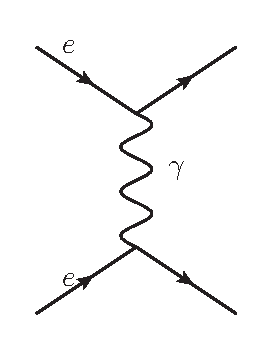
\includegraphics[width=\linewidth,scale=0.5]{figures/scattering.eps}
        \caption{}
        \label{fig:PhotonScattering}
    \end{subfigure}%
    \begin{subfigure}[b]{0.5\textwidth}
        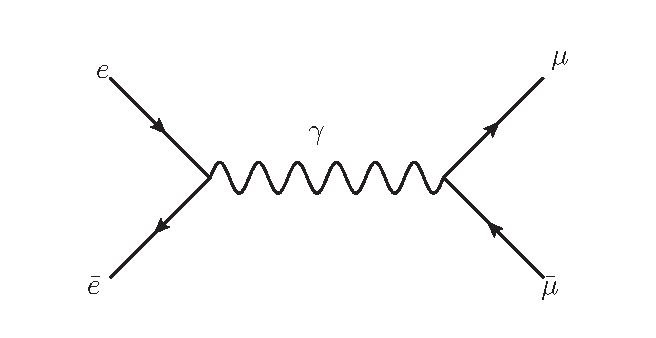
\includegraphics[width=\linewidth]{figures/fermionGammaTrans.eps}
        \caption{}
        \label{fig:FermionPhotonFussion}
    \end{subfigure}% 
    \begin{subfigure}[b]{0.3\textwidth}
        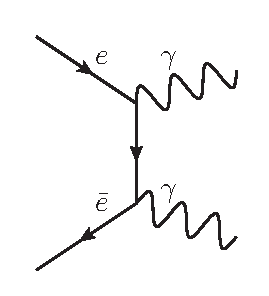
\includegraphics[width=\linewidth]{figures/annailation.eps}
        \caption{}
        \label{fig:PairAnnialation}
    \end{subfigure}%

    \caption[
        Photon interaction examples
    ]{
    Examples of interactions involving the photon. The left figure shows scatter, with two electrons repelling each other. The center demonstrates fusion, with electron/antielectron forming into a photon, which in turn becomes a muon/antimuon pair. The right figure is annihilation, where a electron/antielectron change into a pair of photons.
    }
    \label{fig:PhotonExamples}
\end{figure}

\section{The Strong Force} \label{sec:StrongForce}
This thesis studies particles produced from quarks and is therefore inherently related to the strong force which interacts with them directly. On the scale of an atom, the electromagnetic force can explain many properties of the universe, but it is incapable of explaining the structure of atomic nuclei. Neutrons, being uncharged, should not be bound in the positively charged nucleus; protons, being positively charged, should repel other protons. Thus, if only the electromagnetic force existed, and assuming that the proton was a fundamental particle, the universe would consist solely of hydrogen atoms, i.e. atoms with only one proton. The force responsible for allowing complex nuclei to form is called the strong nuclear force, more simply referred to as just the ``strong force." However, binding nuclei together is merely a residual effect of the strong force; its main function is to bind together the constituent particles that make up neutrons and protons. These particles are called quarks, with protons and neutrons being made of ``up" quarks and ``down" quarks. The proton consists of two up quarks and a down quark, while the neutron is made of two down quarks and an up quark. Similar to electrons, there are two heavier versions of both the up and the down quark, shown in Figure \ref{fig:ParticleTable}. Both the proton and the neutron fall in the overarching classification of a ``hadron," which are particles made up of quarks.\par 

	The strong nuclear force operates by the exchange of ``gluons" between individual quarks, working similarly to the way the exchange of photons cause the electromagnetic force to function. Even so, there are major differences between the two forces. Unlike the electromagnetic force, wherein a particle can have either positive or negative electric charge, the strong force interacts with ``color" charge. This color charge has no relationship to the colors of the electromagnetic spectrum, but rather reflects our familiarity with the term.  The color charge can either be red, blue, or green, and in the case of antiquarks, antired, antiblue, or antigreen. This naming convention was chosen due to the fact that stable combinations of quarks exist in sets such that the ``color" of the set is either ``white" or ``black". This can either be done by having a set of three quarks, with the colors, red, blue and green, creating a white state or a quark/antiquark pair of opposite colors such as blue and antiblue creating a black state. Gluons also carry color charges, allowing them to self-couple; this is unlike a photon, which does not carry electric charge and therefore can not directly interact with other photons. If energy is added to a hadron this energy can be used to create new quark/antiquark pairs. This allows for two quarks to separate while staying in a ``white" ``black" state, since they now have a new quark to bind to. If enough energy was added this can happen multiple times leading to two ``jets" of hadrons going in the direction of the  initial quarks. An example is shown in Fig \ref{fig:JetFormationExample}
	
    
    \begin{figure}[!htbp]
        \centering
        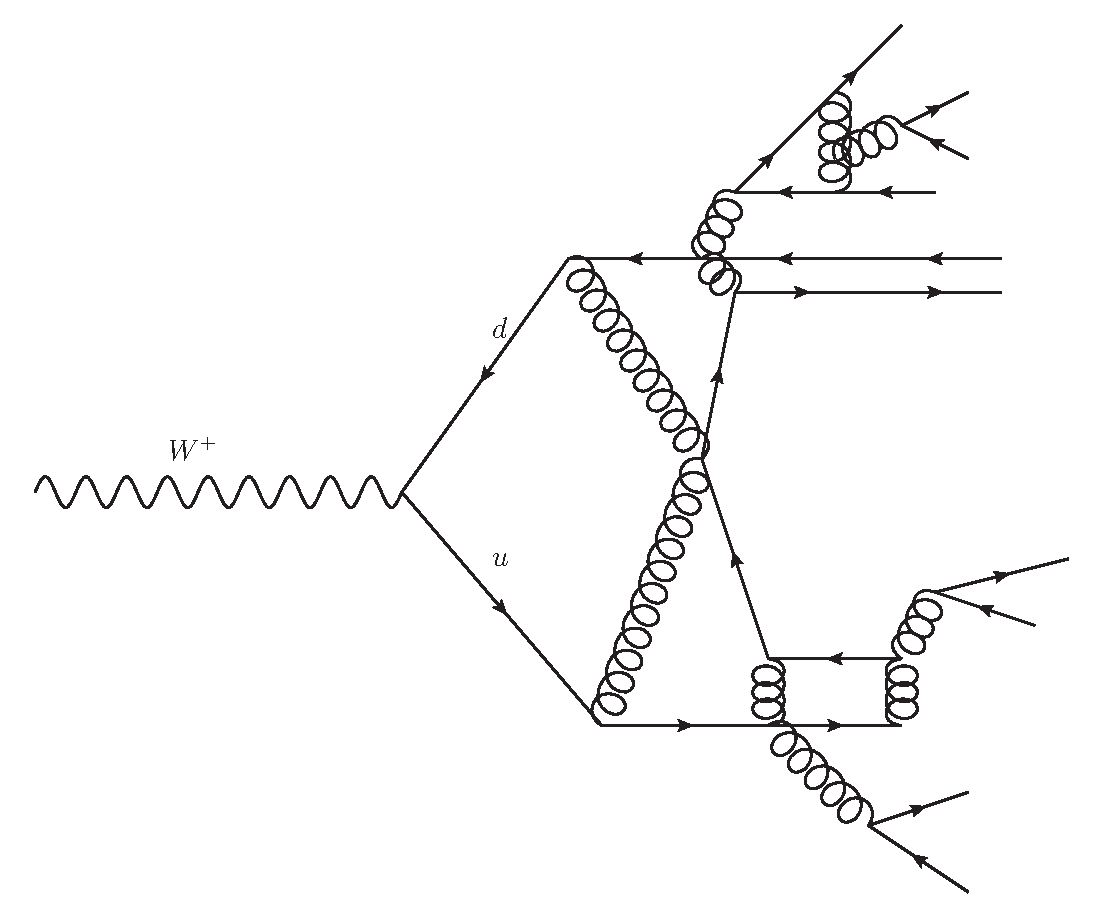
\includegraphics[width=\textwidth]{figures/TheoryFigures/WComplexNew.eps}
        \caption[Jet Formation Example]{A W boson decaying to a quark antiquark pair. due to the excess of energy this leads to the production of multiple new quarks, creating two jets of quarks moving in the direction of the initial proton}
        \label{fig:JetFormationExample}
    \end{figure}{}
    
\section{The Weak Force}
	The weak force interacts with almost all known particles (the exception being the gluon). However, the relative weakness of the force means that these interactions happen at a very low rate. The low rate is primarily due to the fact that all the carriers of the weak force, the two charged bosons W$^+$, W$^-$ and the neutral \Z, have mass, unlike the other two forces. This mass is extremely large compared to the fermions that make up stable matter, being around twenty thousand times heavier than an up or down quark, and two hundred thousand times heavier than a electron. Thus, the rate is so low at usual energy scales experienced by people. that when compared to other exchanges, such as those that use the photon like in Fig \ref{fig:PhotonScattering}, momentum changes due to the weak force interactions are negligible. The only exception in the cases where both the strong and electromagnetic force couplings are suppressed, since in those situations all momentum exchange is due to the weak force. 
	
	Instead, the weak force is known for allowing particles to decay. Unlike both the strong and the electromagnetic forces, which allow a particle/antiparticle pair to change into a different pair, the weak force allows a lone particle to change identity. The typical example given is beta decay as shown in Fig. \ref{fig:NeutronDecay}, where a down quark in neutron decays to a up quark creating a proton, an electron, and an antielectron neutrino. Without this property, particles such as taus and muons would not decay and would only be destroyed when they eventually interact with their respective antiparticles. By contrast, particles like taus and muons do decay on their own, and we only see instances of these particles very shortly after their creation.
    
    The weak force is also the only force that can interact with neutrinos. These particles were first predicted when studying beta decay. When an atom underwent beta decay, the energy of the emitted electron was not a set value. According to the conservation of energy, the energy of the electron should be the mass lost during the decay, which is constant for each decay. Experiments, however, saw that the energy was a continuous distribution. Therefore, it was hypothesized that the energy  was being carried off by an invisible neutral particle. This particle, being neutral in both color and electric charge, did not interact with either the electromagnetic force or the strong force, which made it invisible to detectors at the time. This particle was dubbed the neutrino which has subsequently been observed and subject to much experimental effort.
    
    \begin{figure}[!htbp]
    \centering
    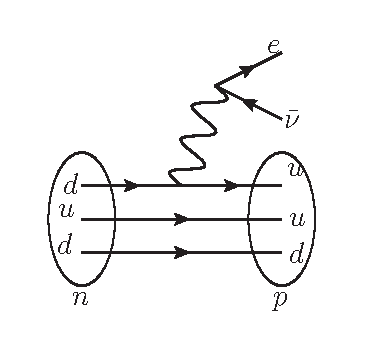
\includegraphics[width=.4\textwidth]{figures/NeutronDecay.eps}
    \caption[
        The particles of the Standard Model.
    ]{
Neutron decay in which a down quark changes to an up quark, as well as an electron and antineutrino.
    }
    \label{fig:NeutronDecay}
\end{figure}
 

 % TODO: Mathematic construction with EM
 
 
  %TOOD This makes strong force c    \caption{}


  
 
 
 \begin{figure}[!htbp]
    \centering
    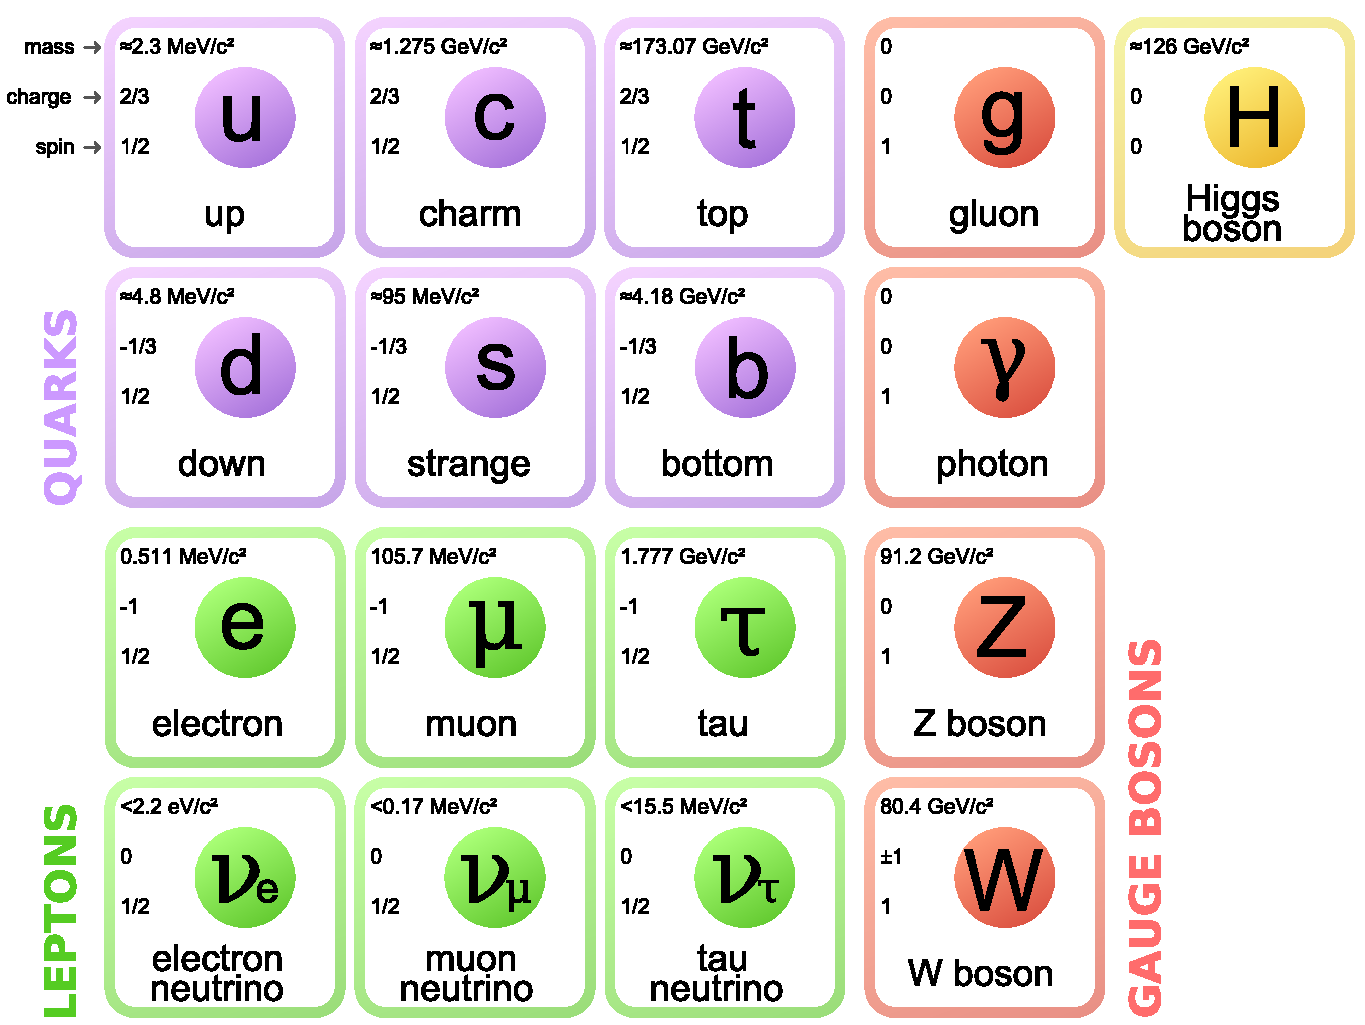
\includegraphics[width=\textwidth]{figures/standard_model.pdf}
    \caption[
        The particles of the Standard Model.
    ]{
      The particles of the Standard Model.
    }
    \label{fig:ParticleTable}
\end{figure}
 
\section{Colliders}


%s, both with themselves and with other particles
The mass of the W is quite large (eighty times the mass of a proton), so powerful are necessary to create the energy to produce them. One type of collider is a lepton collider, such as the Large Electron Positron collider (LEP). Electron colliders are valuable since they produce very clean signals, due to the lack of beam remnants\footnote{Leftover pieces of the proton}. They are restricted, however, by the synchrotron radiation which limits the energy that can be practically achieved. Thus, despite the clarity of the signals, lepton colliders have only discovered the gluon and the tau, as well as helping with the discovery of the charm\cite{TauHistory}\cite{GluonHist}. \par
	Hadron colliders, which come in many types, have been instrumental in discovering many particles and confirming many theories. Due to the higher mass of hadrons compared to electrons, they emit less synchrotron radiation and therefore it is possible to reach higher energies than it would be with a similarly sized lepton collider, which aids the discovery of very massive particles. There are two main ways of  colliding the particles, a two-beam setup and a fixed target. The simplest type is a fixed target. Having a fixed target lowers the possible energies of the interaction, but it drastically increases the luminosity, versus experiments that collide two beams, due to the large density of a solid object compared to the density of a second beam. This type of accelerator was used in the discovery of the bottom quark and the tau neutrino. The other type of hadron colliders collide two beams. These greatly increase the energy of the interaction point. One example is a Proton/Antiproton collider such as the Tevatron and the CERN's Proton-Antiproton Collider. These types of experiments have been used to great success in finding particles of the Standard Model such as the W and the Z bosons, as well as the top quark\cite{ZBosonDiscovery}\cite{Wdiscovery}\cite{WdiscoveryCont}\cite{TopDiscovery}. Another example of a two beam collider is a proton/proton collider. This includes the LHC, which is currently the largest collider in the world. In 2012 the LHC was used to discover the Higgs boson \cite{CMSHiggsPaper} which had been sought unsuccessfully with the Tevatron, among others. Hadron colliders do have a major drawback when compared to lepton colliders, in that collisions always involve beam remnants, leftover pieces of the proton, that complicate analysis of the interactions.\par
    
    
 	At the LHC, one of the main modes of proton/proton interactions producing a W (pp~ $\rightarrow$ W) is shown in Fig \ref{fig:PPWProdcution}.
\begin{figure}[!htbp]
    \centering
    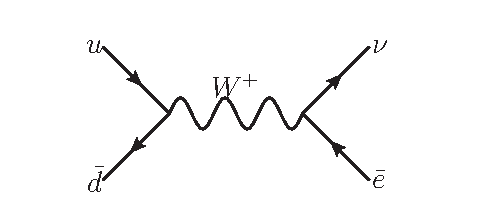
\includegraphics[width=\textwidth]{figures/TheoryFigures/WBosonProduction.eps}
    \caption[
        The particles of the Standard Model.
    ]{
     This is an example of a W$^+$ production in a pp collision.  
 
    }
    \label{fig:PPWProdcution}
\end{figure}
This decay process includes a neutrino, which is undetectable, complicating the mass measurement of the W.  It would be possible to reconstruct the energy of the neutrino by measuring the missing momentum, however the momentum of all other particles in the interaction must be known. Although the momentum of the protons are well known, each quark carries only a fraction of it, and not a constant fraction as the quarks are in constant motion inside the proton. This is further complicated since the leftover quarks, ones not involved in creating the W, are capable of going down the beam pipe, and not interacting with the detector, therefore it is impossible to measure the momentum of these leftover quarks.
	\par In addition to the momentum carried by the real quarks, momentum is carried by the gluons, which hold the quarks together. These gluons are capable of producing new $q\bar{q}$ pairs, which is of particular importance in the production of the W. As was mentioned earlier, protons are classically described as being made of three quarks. In order to create a W, a source of antiquarks is required, in this case gluons. None of this allows for the momentum of the initial particles to be known, removing the possibility of measuring the W mass directly. Instead, in order to calculate the mass of the W, measured events are compared with  an array of simulations that contain different masses. This requires all other aspects of the simulation to be accurately modeled. The uncertainty of many of the components of these simulations, such as the motion of the quarks within the proton, leads to a large uncertainty in the calculated mass of the W which needs to be minimized.
    
    
\subsection{Parton Distribution function}
\label{sec:pdf}
As mentioned in the previous section, quarks within a proton do not carry a constant fraction of the momentum of the proton. The momentum fraction is described using a probability distribution $f_{i}(x_{i};Q^{2})$ with $Q^{2}$ being the energy scale of the interaction, and $x_{i}$ being equal to the fraction of the proton's momentum carried by the particular parton(A gluon or quark making up the proton).  Rather than the intuitive limit 
\begin{equation}
\lim_{Q^{2}\to\infty} f_{i}(x_{i};Q^{2})\approx\delta(x_{i}-1/3)
\end{equation}
that one would expect at high energies, with each of the three real quarks having $1/3$ of the total momentum of the proton as the quark's motion in the proton becomes small compared to the proton's motion in the accelerator. The strong force allows the quarks to drastically change their momentum with respect to each other while staying confined by the exchange of gluons, which also carry momentum. This is further complicated by the gluons splitting into virtual $q\bar q$ pairs\footnote{usually referred to as sea quarks} which also carry momentum.  Unfortunately, the amount of momentum each particle carries is dependent on the strong force's interaction constant, \alphastrong, which varies with Q as can be seen in Fig \ref{fig:alphaStrong}. As can be seen, \alphastrong is larger than one for small values of Q, which makes it impossible to use perturbation theory to calculate $f_{i}(x_{i};Q^{2})$ using first principles. 


\begin{figure}[!htbp]
    \centering
    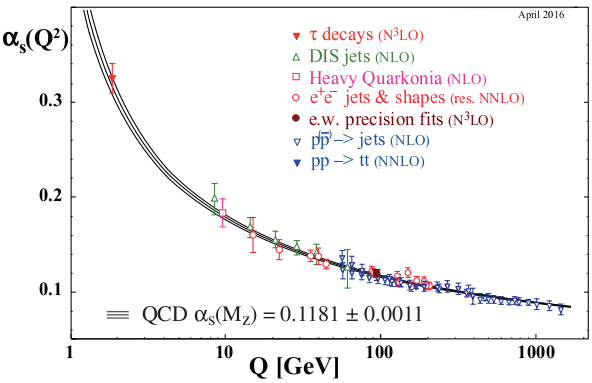
\includegraphics[width=\textwidth]{figures/TheoryFigures/StrongCouplingConstant.png}
    \caption[
      Strong coupling constant 
    ]{
      Strong coupling constant $\alphastrong$ as a function of Q. As can be seen as Q decreases \alphastrong increases, being in the order of 1 for $\SI{1}{GeV}<$ Q $< \SI{10}{GeV}$.
    }
    \label{fig:alphaStrong}
\end{figure}

 Instead $f_{i}(x_{i};Q^{2})$ is calculated based on measurements made at specific values of $Q^{2}$. This function is called the Parton Distribution Function (PDF). Fortunately, although it is not possible to predict PDFs from first principles, it is possible to calculate a PDF at a new $Q^{2}$ based on a previous PDF using the Dokshitzer-Gribov-Lipatov-Altarelli-Parisi(DGLAP) equation \cite{DGLAP1}\cite{DGLAP2}\cite{DGLAP3}\cite{DGLAP4}. Two example PDFs are shown in \cref{fig:PDFExample}. In the left plot, the up and down quarks have a high probability of caring most of the momentum, with a vary low chance of momentum being carried by any of the larger sea quarks. However, as can be seen in the right plot, at higher $Q^2$ there is a much higher chance of a virtual quark, such as a bottom, carry an appreciably fraction of the protons momentum. This is relativly intuitive since at higher energies there is more extra energy for the virtual quark to use to become real.
\iffalse
\begin{equation}\label{eq:alpha_strong}
    \alphastrong \left( Q \right)
    \approx
    \frac{1}{
        \logn \left( Q / \LambdaQCD \right)
    }
\end{equation}
\fi

\begin{figure}[!htbp]
    \centering
    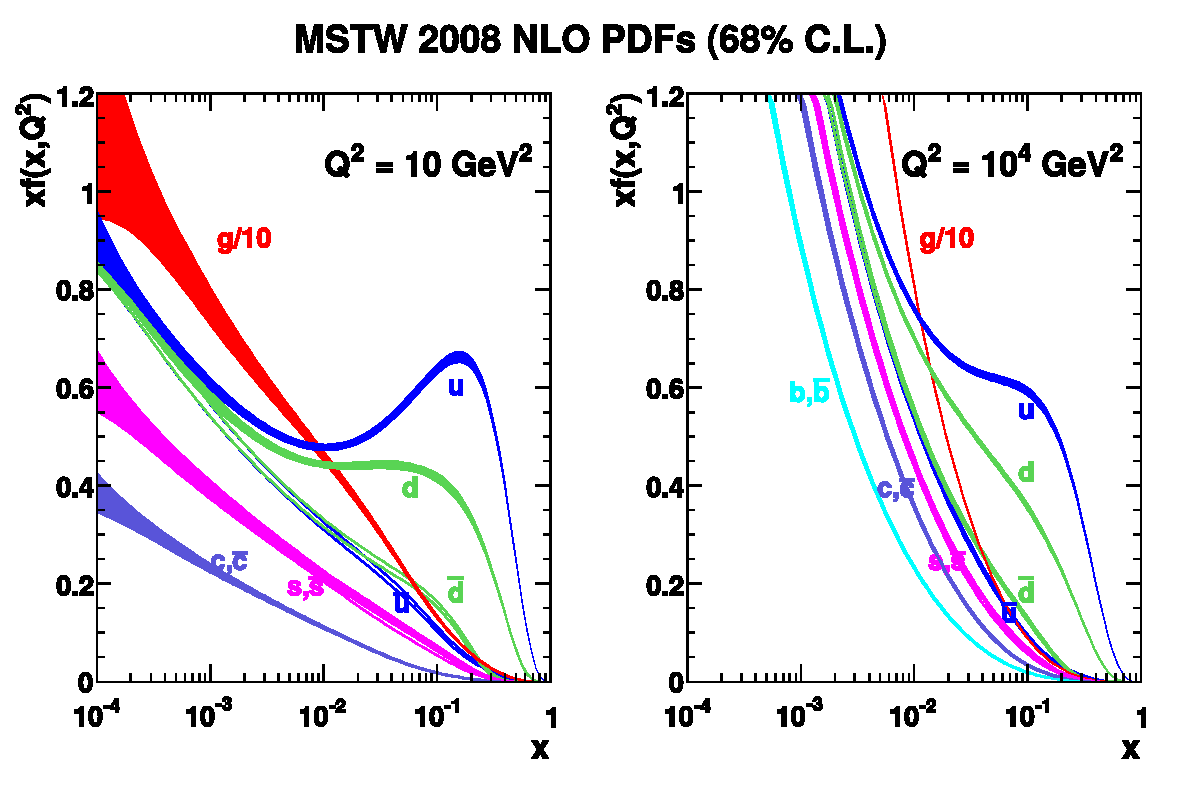
\includegraphics[width=\textwidth]{figures/mstw_pdfs.pdf}
    \caption[
      Parton Distribution Function example
    ]{
      PDF examples for two different Q$^2$ from the MSTW collaboration including confidence levels.   \cite{PDFExample}
    }
    \label{fig:PDFExample}
\end{figure}
 
 \subsection{Kinematics of LHC collisions}
 \label{sec:KinematicsLHC}
At the LHC the center-of-momentum frame for an interaction is not the same as the rest frame for the detector. This complicates measurements of the W since they will then require simulations to account for these effects which, since they are dependant on the strong force, are not predictable through the standard model. It is therefore useful to take measurements that allow us to probe these effects. Although normally a particle produced from two interacting quarks has very little momentum perpendicular to the beam direction, it often carries a large amount of momentum in the direction of the beam. Because of this, it is traditional to use measurements that are Lorentz invariant to a boost along the beam line. These include invariant mass (M) and  momentum perpendicular to the beam line, otherwise known as transverse momentum (\pt). Also useful is rapidity, which is based on the energy(E) of the particle, and its $P_z{}$:
 \begin{equation}\label{eq:RapidityDefinition}
 \rapidity 
 =
 \frac{1}{2}
 \ln
\Bigg(\frac{E+P_{z}}{E-{P_{z}}}\Bigg).
 \end{equation}

Although \rapidity is not Lorentz invariant,  it is still useful because the difference between two rapidities is Lorentz invariant. Although, as mentioned in the previous section, each parton in a proton can have wildly different momenta, it is highly unlikely for them to have a large \pt. Using the assumption that they have neither mass nor transverse momentum, the 4-momenta of the two interacting partons can be described in terms of the center of mass energy of the protons($s$) and the fraction of the momentum carried by the quarks($x_1$ and $x_2$):
 \begin{equation}\label{eq:partonmomentums1}
 p_{1}
 =
 \frac{\sqrt[]{s}}{2}(x_{1},0,0,x_{1}),
\end{equation}
 \begin{equation}\label{eq:partonmomentums2}
 p_{2}
 =
 \frac{\sqrt[]{s}}{2}(x_{2},0,0,-x_{2}).
\end{equation}
Noting the final particle s 4-momentum will be a direct addition of the two quarks 4-momenta it is possible to Use these two four-vectors to write equation \ref{eq:RapidityDefinition} in terms of $x_{1}$ and $x_{2}$.
\begin{equation}\label{eq:RapidityPDF}
\rapidity
=
\ln
\Big(\frac{x_{1}}{x_{2}}\Big).
\end{equation}
It is then possible to describe $x_{1}$ and $x_{2}$ in terms of \rapidity, $M$, and $s$ as

\begin{equation}\label{eq:BjorkeninY}
x_{1,2}
=
\frac{M}{\sqrt[]{s}}
e^{\pm \rapidity}.
\end{equation}This is useful because, although we cannot measure the momentum of the partons, we are able to use measurable quantities of the interaction (in this case the mass and the rapidity) to calculate the momentum of the initial particles.

 
 \section{Understanding the initial conditions in hadron collisions}\label{sec:probingQCD}
Understanding the quarks that are involved in the production of particles of interest in hadron collisions is vital for tests of the Standard Model that use them. Although it is possible to calculate many different hard interactions for different energies of quarks, this calculation can not predict final results without knowledge of the quarks making up the proton. Therefore, studying these initial conditions of a proton are necessary to do analysis that use proton collisions.
 \subsection{Importance of probing QCD for measuring mass of the W Boson}
As outlined above, measuring the mass of the W boson ($M_{W}$) accurately is difficult to do in hadron colliders, which makes it difficult to test whether the difference between the theoretical mass and the measured mass is due to a measurement error or an issue with the SM. The W's most common decay, $W \rightarrow q\overline{q}$ creates two jets. In hadron colliders, the strong force produces jets at high enough rates that it is not practical to attempt use them to measure electroweak physics(sec.\ref{Sec:Trigger}). Therefore the best decay channel for measuring $M_{W}$ is $W\rightarrow l\nu$. In this technique the \pt of the lepton is compared to simulations, with an example shown in Fig \ref{fig:WPtlPlot}. This, however, requires that the \pt of the W itself is accurately modeled. This is difficult since QCD interactions that boost the W by relevant amounts must be accurately modeled, but are impossible to predict using the SM. Since this model is not based on a calculable theory but rather attempts to fit data, it inherently can bring uncertainty into the system if the area being probed is not near where the model was based.
\begin{figure}[!htbp]
    \centering
    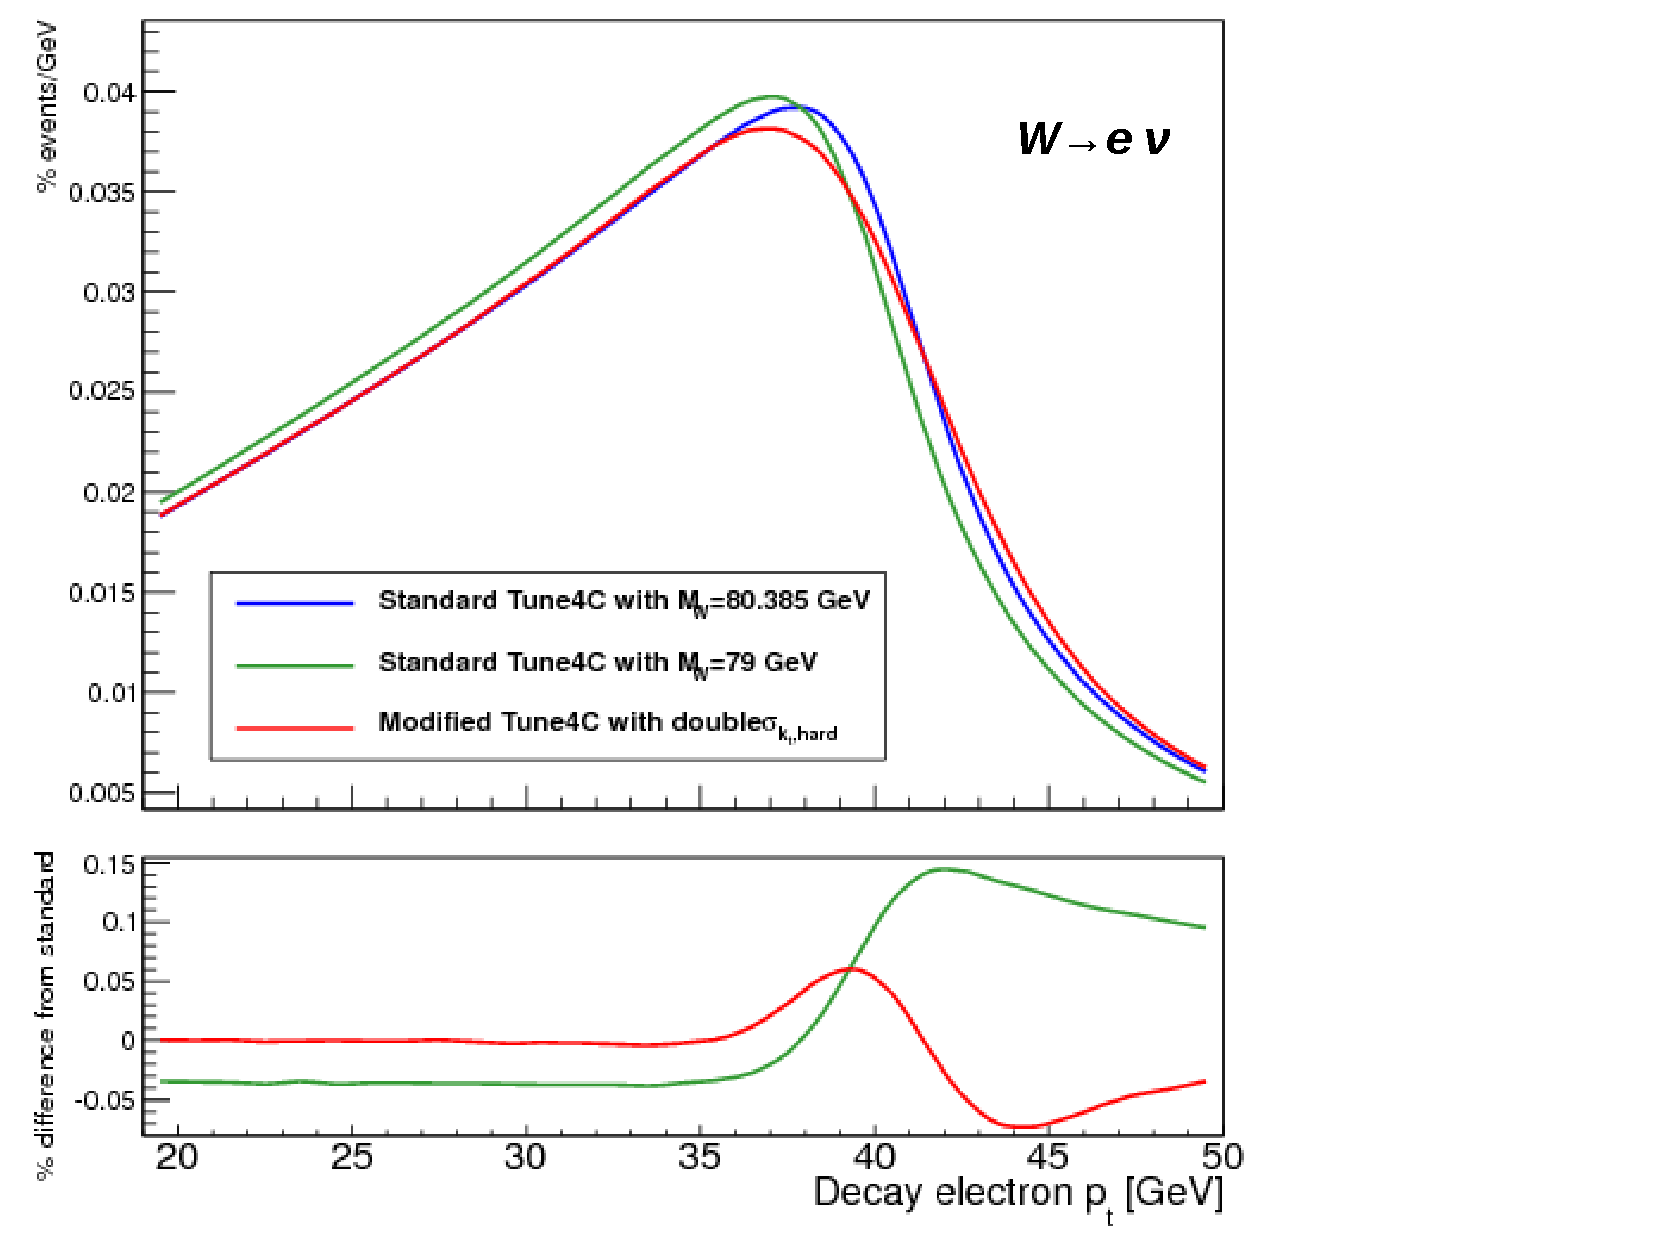
\includegraphics[width=\textwidth]{figures/TheoryFigures/WPtCompare.pdf}
    \caption[
      W boson lepton \pt
    ]{
   W boson lepton \pt of multiple simulated W bosons with changes to the W mass as well as other simulation settings.
     
    }
    \label{fig:WPtlPlot}
\end{figure}


\subsection{Next-to-leading order production}
\label{sub:QCDimportance}
Although, as can be seen in Fig \ref{fig:alphaStrong}, \alphastrong is smaller than unity at energies that produce a weak vector boson, allowing for a solution to be solved perturbatively, this is not practically feasible. This is due to the large value of \alphastrong at a value of $\approx$ 0.3, which would require at least 8th-order effects to be calculated to get the required accuracy. This is not practical with current technology. Instead, the current simulation makes next-to-leading order (NLO) corrections to the cross-section that come with the strong-coupling directly, and a hadronizer simulates the higher order effects. These include situations that have extra terms in the final state as well as gluon loops.
The emission of a parton during the process is of particular importance in the calculation of transverse momentum. One possible emission is a single gluon, as is shown in Fig. \ref{fig:feyn_DYISR}. This emission can give the quark a transverse momentum. Because \alphastrong increases at low energies, these gluons tend to have small momenta, so usually contribute small amounts of momentum to the boson. Thus, it is quite important to accurately model when comparing the low momentum vector bosons in data. Figure \ref{fig:feyn_DYQuarkRadiation} shows a quark emitting a vector boson and interacting with a gluon. Unlike the case when the gluon is emitted, the quark can have a large momentum and generate a vector boson with a larger transverse momentum. Such an interaction can be accurately predicted by perturbation QCD calculations.
\begin{figure}[!p]
    \centering
    \begin{subfigure}[b]{\SideBySidePlotWidth}
        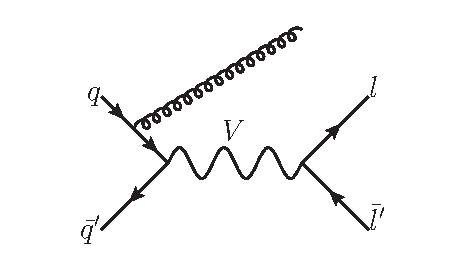
\includegraphics[width=\linewidth]{figures/TheoryFigures/VectorBosonQToLeptonGJet.eps}
        \caption{}
        \label{fig:feyn_DYISR}
    \end{subfigure}%
    \begin{subfigure}[b]{\SideBySidePlotWidth}
        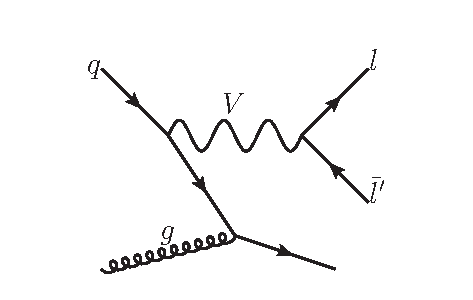
\includegraphics[width=\linewidth]{figures/TheoryFigures/VectorBosonQToLeptonqJet.eps}
        \caption{}
        \label{fig:feyn_DYQuarkRadiation}
    \end{subfigure}%
    \hfill
    \begin{subfigure}[b]{\SideBySidePlotWidth}
        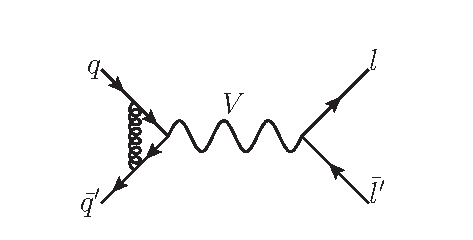
\includegraphics[width=\linewidth]{figures/TheoryFigures/VectorBosonQToLeptonqgexchange.eps}
        \caption{}
        \label{fig:feyn_DYloops}
    \end{subfigure}%
    \begin{subfigure}[b]{\SideBySidePlotWidth}
        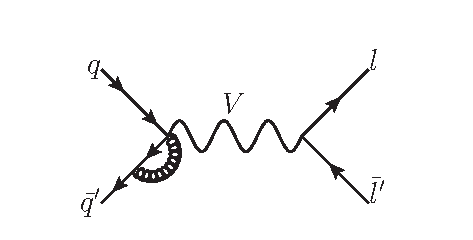
\includegraphics[width=\linewidth]{figures/TheoryFigures/VectorBosonQToLeptonqLoop.eps}
        \caption{}
        \label{fig:feyn_DYmoreloops}
    \end{subfigure}%

    \caption[
        Higher order DY Feynman diagrams.
    ]{
        Higher order DY Feynman diagrams. a is an example of when an incoming quark radiates a gluon. In b the quark radiates a \Z before interacting with a gluon. In both c and d the gluons interact with the quarks but are not radiated.
    }
    \label{fig:higher_order_z_diagrams}
\end{figure}



\begin{figure}[!p]
    \centering
    \begin{subfigure}[b]{\SideBySidePlotWidth}
    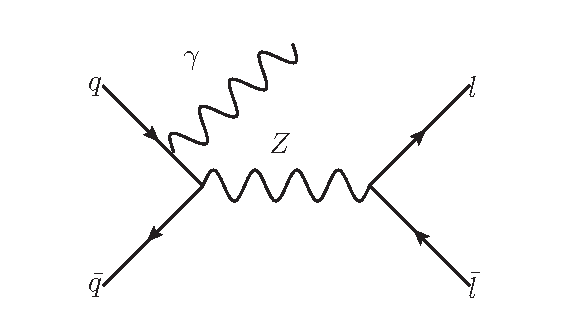
\includegraphics[width=\linewidth]{figures/TheoryFigures/ISRExample.eps}
    \caption{}
    \end{subfigure}%
        \begin{subfigure}[b]{\SideBySidePlotWidth}
    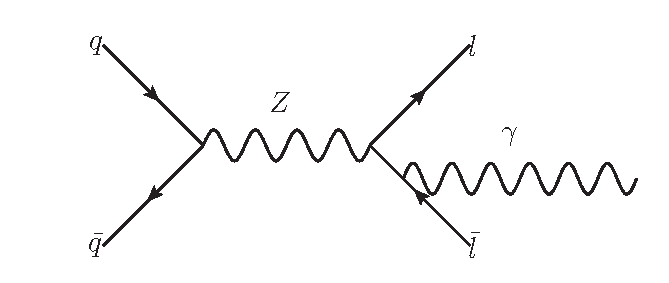
\includegraphics[width=1.1\linewidth]{figures/TheoryFigures/FSRExample.eps}
    \caption{}
    \end{subfigure}%
    \caption[FSR and ISR example]{On the left is an example ISR in which one of the initial quarks produces a photon before fusing into a Z. The right plot shows a FSR example in which one of the leptons produced emits a photon.}
    \label{fig:ISRFSR}
\end{figure}
 \subsection{Using the \Z Boson to more accurately measure QCD interactions}

The Drell-Yan (DY) process produces a pair of leptons from the annihilation of a quark-antiquark pair in a hadron-hadron collision - a process that is almost exactly the same as W production in Fig \ref{fig:DYSimple}. However, the Drell-Yan process differs in that both its final products are detectable which allows for direct measurements of the \Z unlike the W. This allows all aspects of the prediction, such as the $Q_T$, to be compared to data with more precision than can be achieved using measurements of the W. By improving the accuracy of the \Z simulation, the accuracy of the W can also be improved.
 \begin{figure}[!htbp]
    \centering
    \begin{subfigure}[b]{\SideBySidePlotWidth}
        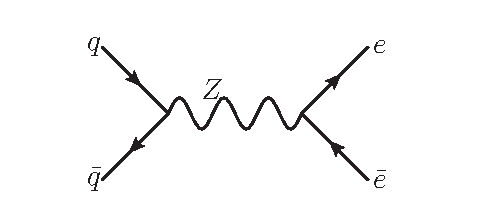
\includegraphics[width=\linewidth]{figures/DYSimple.eps}
        \caption{}
        \label{fig:feyn_DYSimpleLeft}
    \end{subfigure}%
    \begin{subfigure}[b]{\SideBySidePlotWidth}
        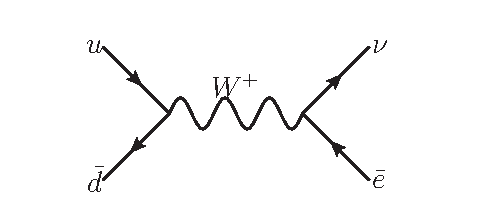
\includegraphics[width=\linewidth]{figures/TheoryFigures/WBosonProduction.eps}
        \caption{}
        \label{fig:feyn_WBosonProduction}
    \end{subfigure}%
    \caption[
      Fenymen diagrams of V\rightarrow\xxbar{l}{l}
    ]{
    Fenymen diagrams showing quarks going to leptons. The left plot shows a quark pair going to a charged pair of leptons while the right plot shows a pair of quarks using a W to become a positron and an antineutrino.
     
    }
    \label{fig:DYSimple}
\end{figure}



\subsection{Photon Emission}
\label{sec:StateRad}
Despite the fact that the photon does not couple directly with the Z boson, it can either affect the measurement of the Z or the production of the \Z itself. The most obvious examples are the case of Initial State Radiation(ISR) and Final State Radiation(FSR), both of which are shown in Fig \ref{fig:ISRFSR}. FSR is of particular importance for this study since the photon carries off some of the energy of the leptons. This can cause inaccurate measurements of the vector bosons \bosonpt since the decay products are used to calculate the properties of the vector boson. Happily, existing perturbation techniques are well-adapted to the necessary precision in this case.




%\begin{figure}[!p]
    \centering
    \begin{subfigure}[b]{\SideBySidePlotWidth}
        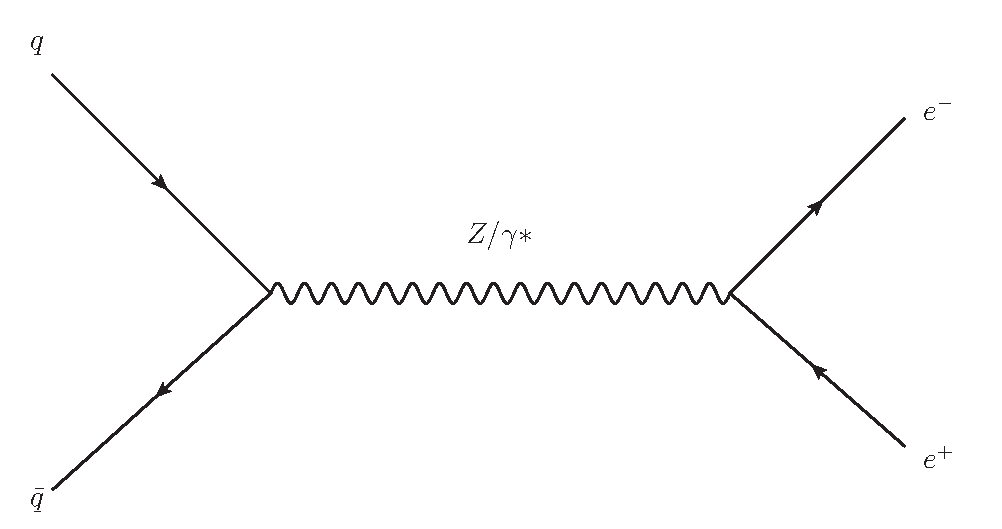
\includegraphics[width=\linewidth]{figures/NormalDY.eps}
        \caption{}
        \label{fig:feyn_qqbar_to_zg}
    \end{subfigure}%

    \caption[
        Higher order in \alphastrong \Ztoee Feynman diagrams.
    ]{
        fill
    }
    \label{fig:LowerOrder}
\end{figure}

 
\subsection{Indirect measurements of \texorpdfstring{$\bosonpt$}{Bosonpt}  using \texorpdfstring{\phistar}{Phistar}}
\label{subsec:Phistar}
With the current detector measurements, the energy of the electron has uncertainties of the order 1\% due to systematics, as well as detector resolution. This leads to measurements of the Z having resolutions on the order of a GeV.  As mentioned in Sec. \ref{sub:QCDimportance}, QCD radiation can give the vector boson a small boost in the transverse direction. For this reason, it is useful to compare the models to the data in the low $Q_{T}$ region. However, the uncertainty of the measurements are of the order of the measurements themselves. Rather then measuring the \bosonpt directly, theorists have proposed using a variable named \phistar\cite{PhiStarSource}. The variable \phistar is correlated with \bosonpt as can be seen in Fig \ref{fig:QtToPhiStar}. In this figure events tend to fall into bins that are in the diagonal with fewer events as you get farther from it. This demonstrates a high, simple correlation between the two variables with high \bosonpt implying a high \phistar and more importantly a low \bosonpt implying a \Z with a low \phistar.
\begin{figure}[!htbp]
    \centering
    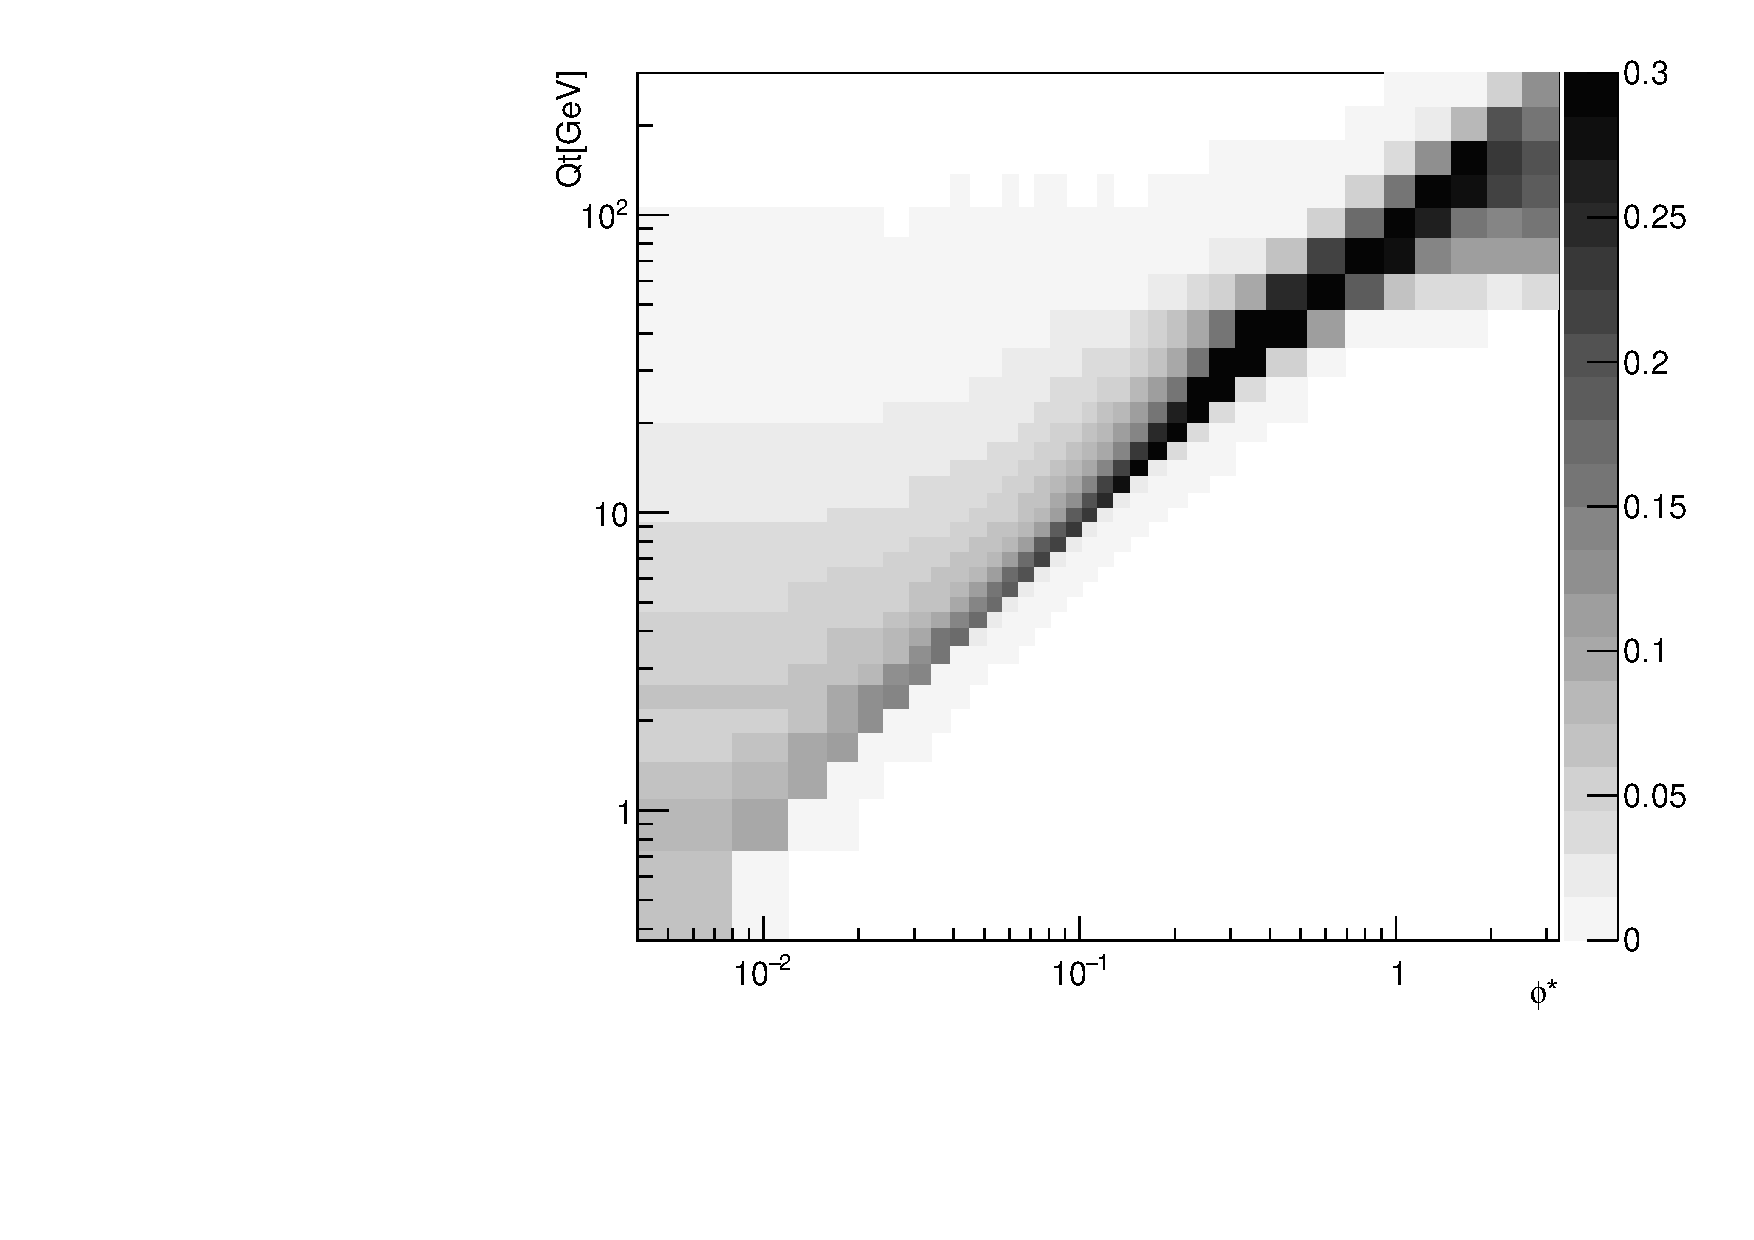
\includegraphics[width=\textwidth]{figures/TheoryFigures/Normalized.pdf}
    \caption[
      \phistar to \bosonpt histogram
    ]{
   Two dimensional plot showing the correlation between \phistar and \bosonpt of the \Z. A relationship between the two is clear with a strong diagonal line down the two dimensional histogram showing a high degree of corrilation between the two variables
     
    }
    \label{fig:QtToPhiStar}
\end{figure}
The definition of \phistar is
\begin{equation}\label{eq:Phistar}
\phistar
=
\cot\frac{\Delta\phi}{2}\sech\frac{\Delta\eta}{2},
\end{equation}
where $\Delta\phi$ is the azimuthal opening angle between the leptons, and $\Delta\eta$ is the angle of the leptons with respect to the beam line in the rest frame of the dilepton pair.  The variable \phistar can  be measured precisely when compared to \bosonpt because the accuracy of the measurements of position and direction inside the CMS detector are, in general, more accurate than the measurements of energy. As can be seen from Fig \ref{fig:QtToPhiStarError}, the relative error in reconstruction of $Q_{T}$ to its generated value is much larger than in the case of \phistar, with the majority of events of \phistar having errors below 5\%.

\begin{figure}[!htbp]
    \centering
    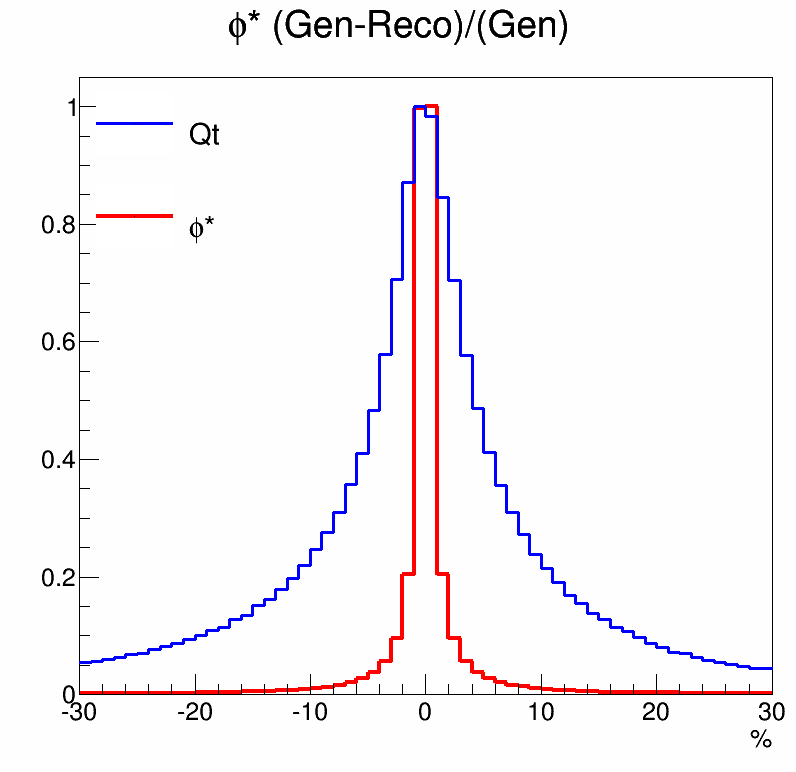
\includegraphics[width=\textwidth]{figures/TheoryFigures/PhistarAndQtPercentageError.png}
    \caption[
      Relative error in phi* and $Q_{T}$ measurements
    ]{
Relative error in phi* and $Q_{T}$ measurements. The measurement of \phistar tends to have a relative error between the reconstructed and the generated value of a couple percentage points while the \bosonpt has an appreciable percentage of events over 20\%.
     
    }
    \label{fig:QtToPhiStarError}
\end{figure}

This variable has been measured by multiple different groups at different center of mass energies. This includes two measurements at the LHC: one by CMS at center-of-mass energy of 8 TeV\cite{PhistarAnMINE}, as well as one by ATLAS (another experiment at the LHC), which measured \phistar at center-of-mass energy of 7~TeV \cite{PhistarAnAtlas}. D0 also measured \phistar at the Tevatron at center-of-mass of 1.96~GeV \cite{PhistarAn1}\cite{PhistarAn2}. However, each of these shows a difference between simulations and data that can not be explained by systematic errors. This thesis presents an attempt to tune the simulation to match the 8~TeV CMS data.

 
%%%%%%%%%%%%%%%%%%%%%%%%%%%%%%%%%%%%%%%%%%%%%%%%%%%%%%%%%%%%%%%%%%%%%%%%%%%%%%%%

%%%%%%%%%%%%%%%%%%%%%%%%%%%%%%%%%%%%%%%%%%%%%%%%%%%%%%%%%%%%%%%%%%%%%%%%%%%%%%%%
